\documentclass[12pt]{extbook}

% \usepackage[paperwidth=5.5in, paperheight=8.5in, margin=0.3in]{geometry}
% \usepackage[paperwidth=8.5in, paperheight=11in, margin=0.5in]{geometry}

\usepackage[paperwidth=8.5in, paperheight=8.5in,bindingoffset=0.125in,margin=0.8in]{geometry}

\usepackage{tikz}

\newcommand{\gl}[2]{
  \begin{center}  
    \resizebox{15cm}{!}{%
      \begin{tikzpicture}[inner sep=7mm]

      \def\lines{#1}  
      \def\linesMinusOne{#2}  

      \draw[help lines, color={gray!20}] (-6,-\lines) grid (6,\lines);

      \foreach \y in {-\lines,...,\linesMinusOne}
        {\draw[-, thick] (-6,\y) -- (6,\y);}

      \end{tikzpicture}
    } 
  \end{center}
}

% Fonts and typography

%% Typography
\usepackage[no-math]{fontspec}
\defaultfontfeatures{Mapping = tex-text, Scale = MatchLowercase}

\usepackage{csquotes}

%% Fonts
%\setmainfont{Adobe Garamond Pro}
%\setsansfont{Adobe Garamond Pro}
\setmonofont[Mapping=tex-ansi]{Menlo}

\newfontfamily\coder[Mapping=tex-ansi]{Menlo}

%% Set Sans font in headings
% \usepackage{sectsty}
% \allsectionsfont{\sffamily}

%% Set polyglossia language
\usepackage{polyglossia}
\setdefaultlanguage{english}

% \usepackage[fontsize=16pt]{scrextend}

\usepackage{titlesec}
% \titleformat{\chapter}[display]
%   {\normalfont\sffamily\huge\bfseries\centering}
%   {\chaptertitlename\ \thechapter}{20pt}{\Huge}
\titleformat{\section}
  {\normalfont\sffamily\huge\bfseries\centering}
  {\thesection}{1em}{\Huge}
% \titlespacing*{\chapter}{0pt}{30pt}{20pt}

% \usepackage{titlesec}
% \titleformat{\chapter}[display]
% {\normalfont\huge\bfseries}{\centering\chaptertitlename\ \thechapter}{20pt}{\Huge}


% new page for every chapter
% \newcommand{\sectionbreak}{\clearpage}

% Page

%% Use full page in book style
% \usepackage{fullpage}

\usepackage{fancyhdr}
\pagestyle{fancy}
\fancyhf{}
\fancyhead{}
\fancyfoot{}
\renewcommand{\headrulewidth}{0.1pt}
% \headrulewidth 0.0pt
% \fancyfoot[C]{\thepage}
\fancyfoot[RO, LE] {\thepage}

%% Set line spacing
\usepackage{setspace}
\setstretch{1.2}

%% Disable paragraph indentation
\usepackage{parskip}

\usepackage{afterpage}

\newcommand\blankpage{%
    \null
    \thispagestyle{empty}%
    \addtocounter{page}{-1}%
    \newpage}


%% Start sections from new page
% \let\stdsection\section
% \renewcommand\section{\newpage\stdsection}

\usepackage[labelformat=empty]{caption}

% Images
\usepackage{graphicx}

\usepackage{pdfpages}

\usepackage{wallpaper}
%\usepackage{everyshi,eso-pic,calc,ifthen,wallpaper}
\usepackage{xcolor}

%% Tango color scheme
\definecolor{SkyBlue}{HTML}{3465A4}
\definecolor{DarkSkyBlue}{HTML}{204A87}

\definecolor{Plum}{HTML}{75507B}

\definecolor{ScarletRed}{HTML}{CC0000}

\definecolor{Aluminium1}{HTML}{EEEEEC}
\definecolor{Aluminium6}{HTML}{2e3436}

\definecolor{Black}{HTML}{000000}

\definecolor{Grayr}{HTML}{777777}


\usepackage{listings}

\lstdefinelanguage{CODER}{%
  morekeywords = {PAU, JLS, OUIMTQ, ZSMELC, LP, ELJT, L, OLE, ELC, ZRS, XRSP, IRRETUJQ, IRRE, VLXPLMTQ, LTE, XMSLPUQ},
  ndkeywords = {class, export, boolean, throw, implements, import, this},
  % ndkeywordstyle = \color{Aluminium6}\bfseries,
  % identifierstyle = \color{Black},
  sensitive = false,
  comment = [l]{//},
  morecomment = [s]{/*}{*/},
  % commentstyle = \color{Plum}\ttfamily,
  stringstyle = \color{ScarletRed}\ttfamily,
  morestring = [b]',
  morestring = [b]"
}

\lstset{
  language = CODER,
  % backgroundcolor = \color{Aluminium1},
  extendedchars = true,
  basicstyle = \normalsize\ttfamily,
  showstringspaces = false,
  showspaces = false,
  tabsize = 1,
  breaklines = true,
  keywordstyle=\color{Grayr},
  showtabs = false
}

%% Normal enumerates processing
% \usepackage{enumerate}

%% Disable section numbers
% \setcounter{secnumdepth}{0}

\renewcommand\thesection{\arabic{section}}

\begin{document}

  % Title page
  % \thispagestyle{empty}
  % \pagestyle{myheadings}
  % \vspace*{\fill}
  %   \begin{center}
  %     \includegraphics[width=\textwidth][width=0.98\textwidth]{img/title}
  %   \end{center}
  % \vspace*{\fill}

  % \begin{figure}
  % \noindent\makebox[\textwidth][c]{\includegraphics[width=\textwidth][width=1.4\textwidth]{img/title}}%
  % \end{figure}

  % \includepdf[pages={1}]{img/captain_z_title_2.pdf}

  \pagestyle{empty}
  \vspace*{\fill}
  \begin{center}
%   \ThisCenterWallPaper{1}{img/cover.png}
   \ThisLLCornerWallPaper{2}{img/cm-cover.png}
   \ThisULCornerWallPaper{1}{img/cm-cover.png}

%    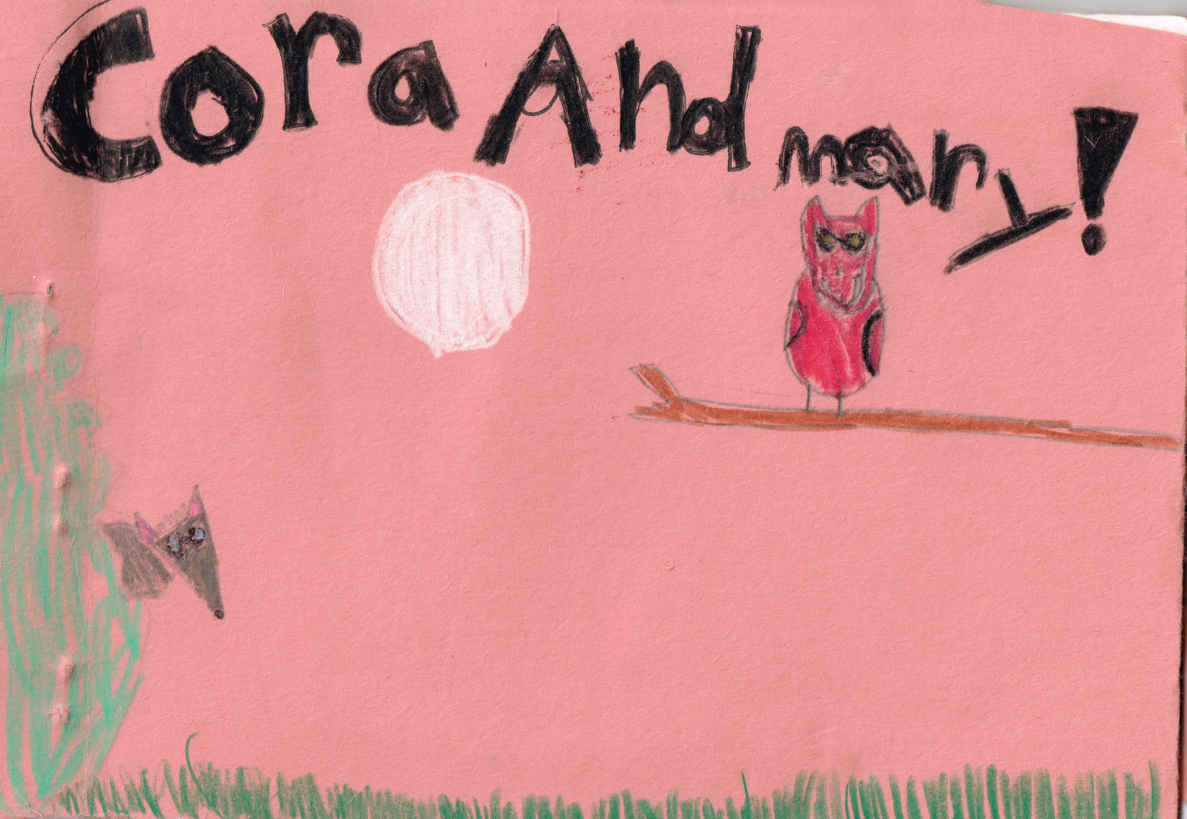
\includegraphics[width=\textwidth]{img/cover.png}  
  %\huge{Cora and Mary}\\[0.5cm]
  \end{center}
  \vspace*{\fill}
  % \afterpage{\blankpage}
  % \clearpage

  \begin{titlepage}
    \vspace*{\fill}
    \begin{center}
      \huge{Cora and Mary}\\[0.5cm]
      \large {E. M. Stone}\\[0.4cm]
      \large {\textit{Illustrated by} E. M. Stone}\\[0.4cm]
    \end{center}
    \vspace*{\fill}
  % \clearpage
  \end{titlepage}
  
  \begingroup
  \footnotesize
  \parindent 0pt
  \parskip \baselineskip
  \vfill
  Cora and Mary \\
  E. M. Stone \\


  Copyright \textcopyright{} 2016 by E. M. Stone \\
  
  All rights reserved. No part of this publication may be reproduced, stored in a retrieval system, or transmitted in any form or by any means without prior written permission of the copyright owners. 
  
%  If you want permission, just let me know.\\
%  Contact information can be found at vallandingham.me


  ISBN-13: 978-1541071926\\
  ISBN-10: 1541071921 

  First edition: December 2016

  \vfill
%  vallandingham.me\\
%  captainZbook.com
  \vspace*{2\baselineskip}
  \clearpage
  \endgroup

  \begingroup
  \vspace*{\fill}
  \begin{center}
  To Cora and Mary.
  \end{center}
  \vspace*{\fill}
  \afterpage{\blankpage}
  \endgroup
  \setcounter{page}{0}
  \clearpage
  

  % \frontmatter
  
  \pagestyle{fancy}

\LARGE
  % Book contents
%\begin{center}
%  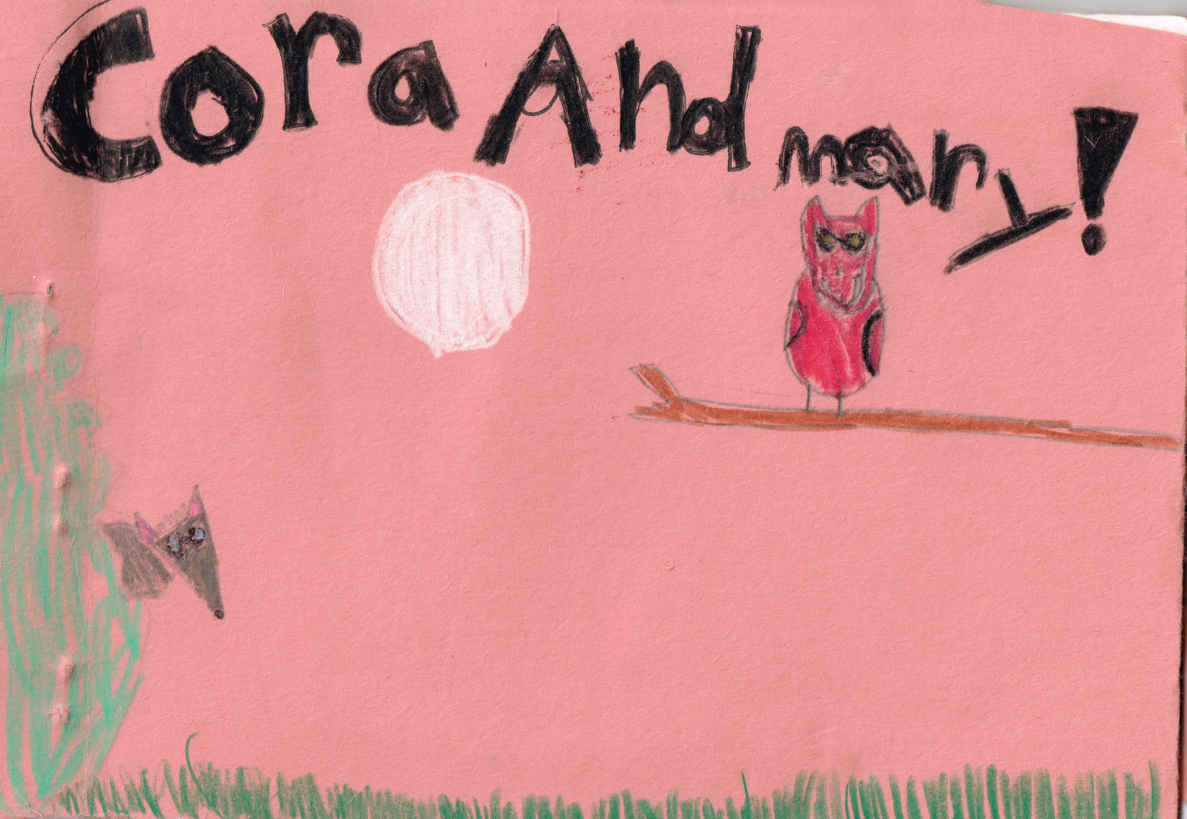
\includegraphics[width=\textwidth]{img/cover.png}
%\end{center}

  Once upon a time, there lived an owl. Her name was Cora. She had a
  unique birthmark. Her birthmark was a black patch around her eyes that
  looked like a mask. None of the neighbor owls wanted to be friends with
  her because they thought her birthmark was ugly. They didn't even want
  to look at her. Cora was very lonely.

\begin{center}
  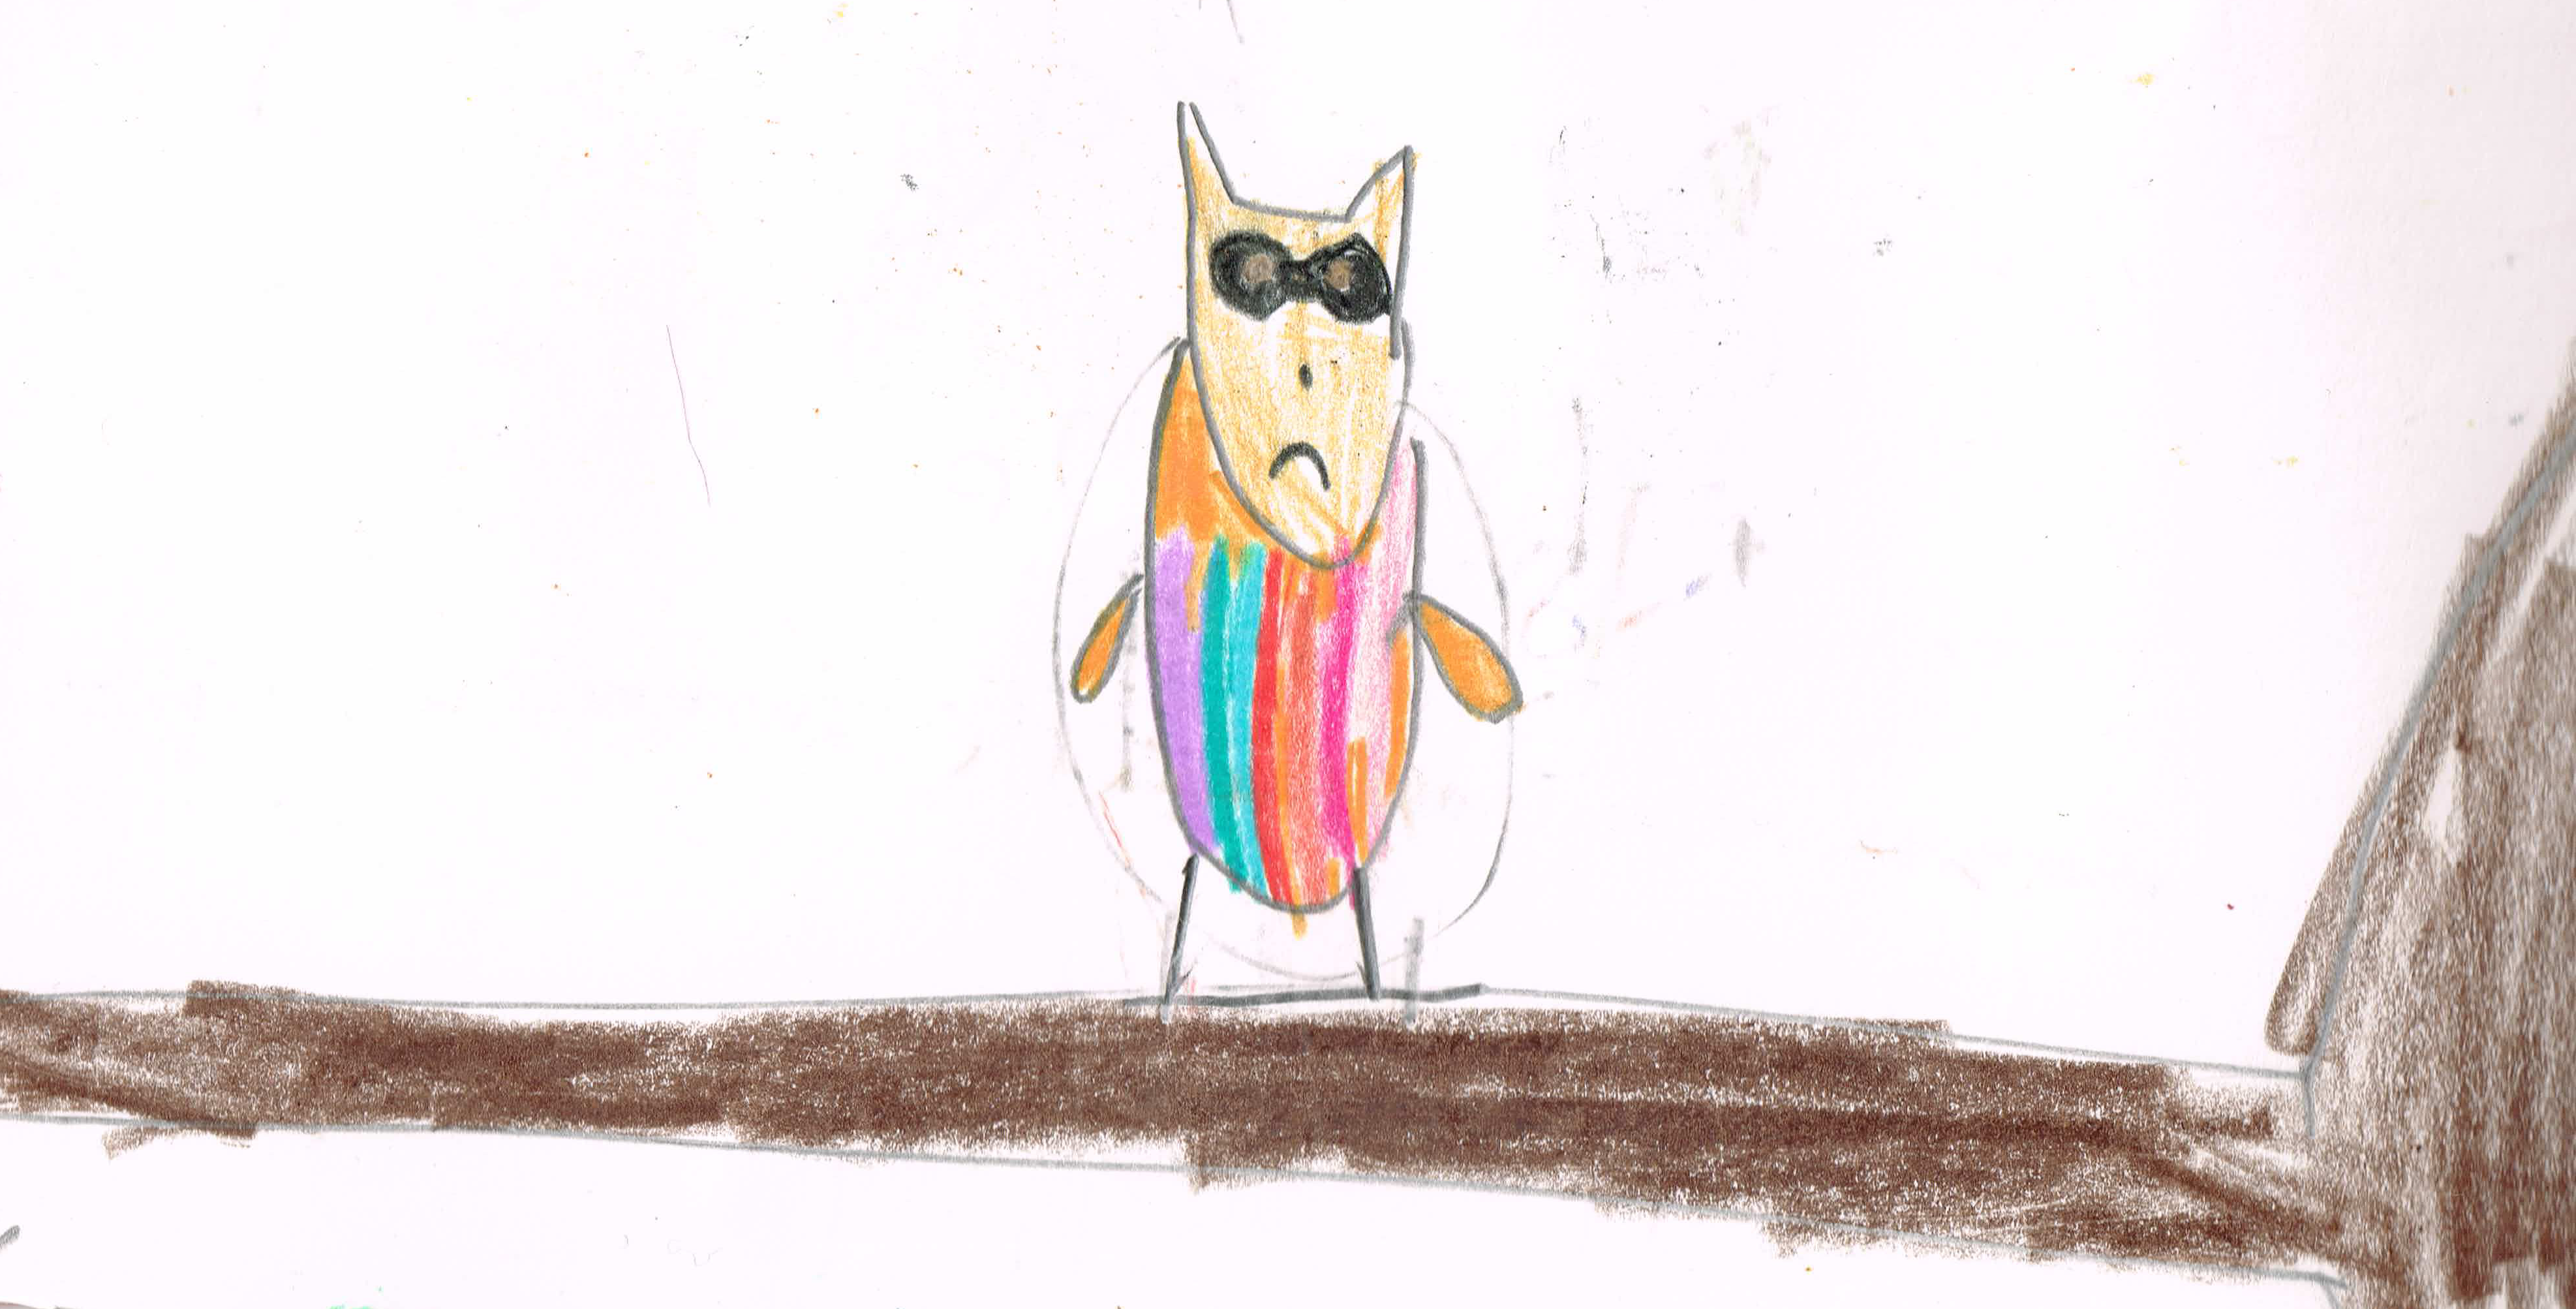
\includegraphics[width=\textwidth]{img/cm-pic01.png}
\end{center}
  
\pagebreak
  
\begin{center}
  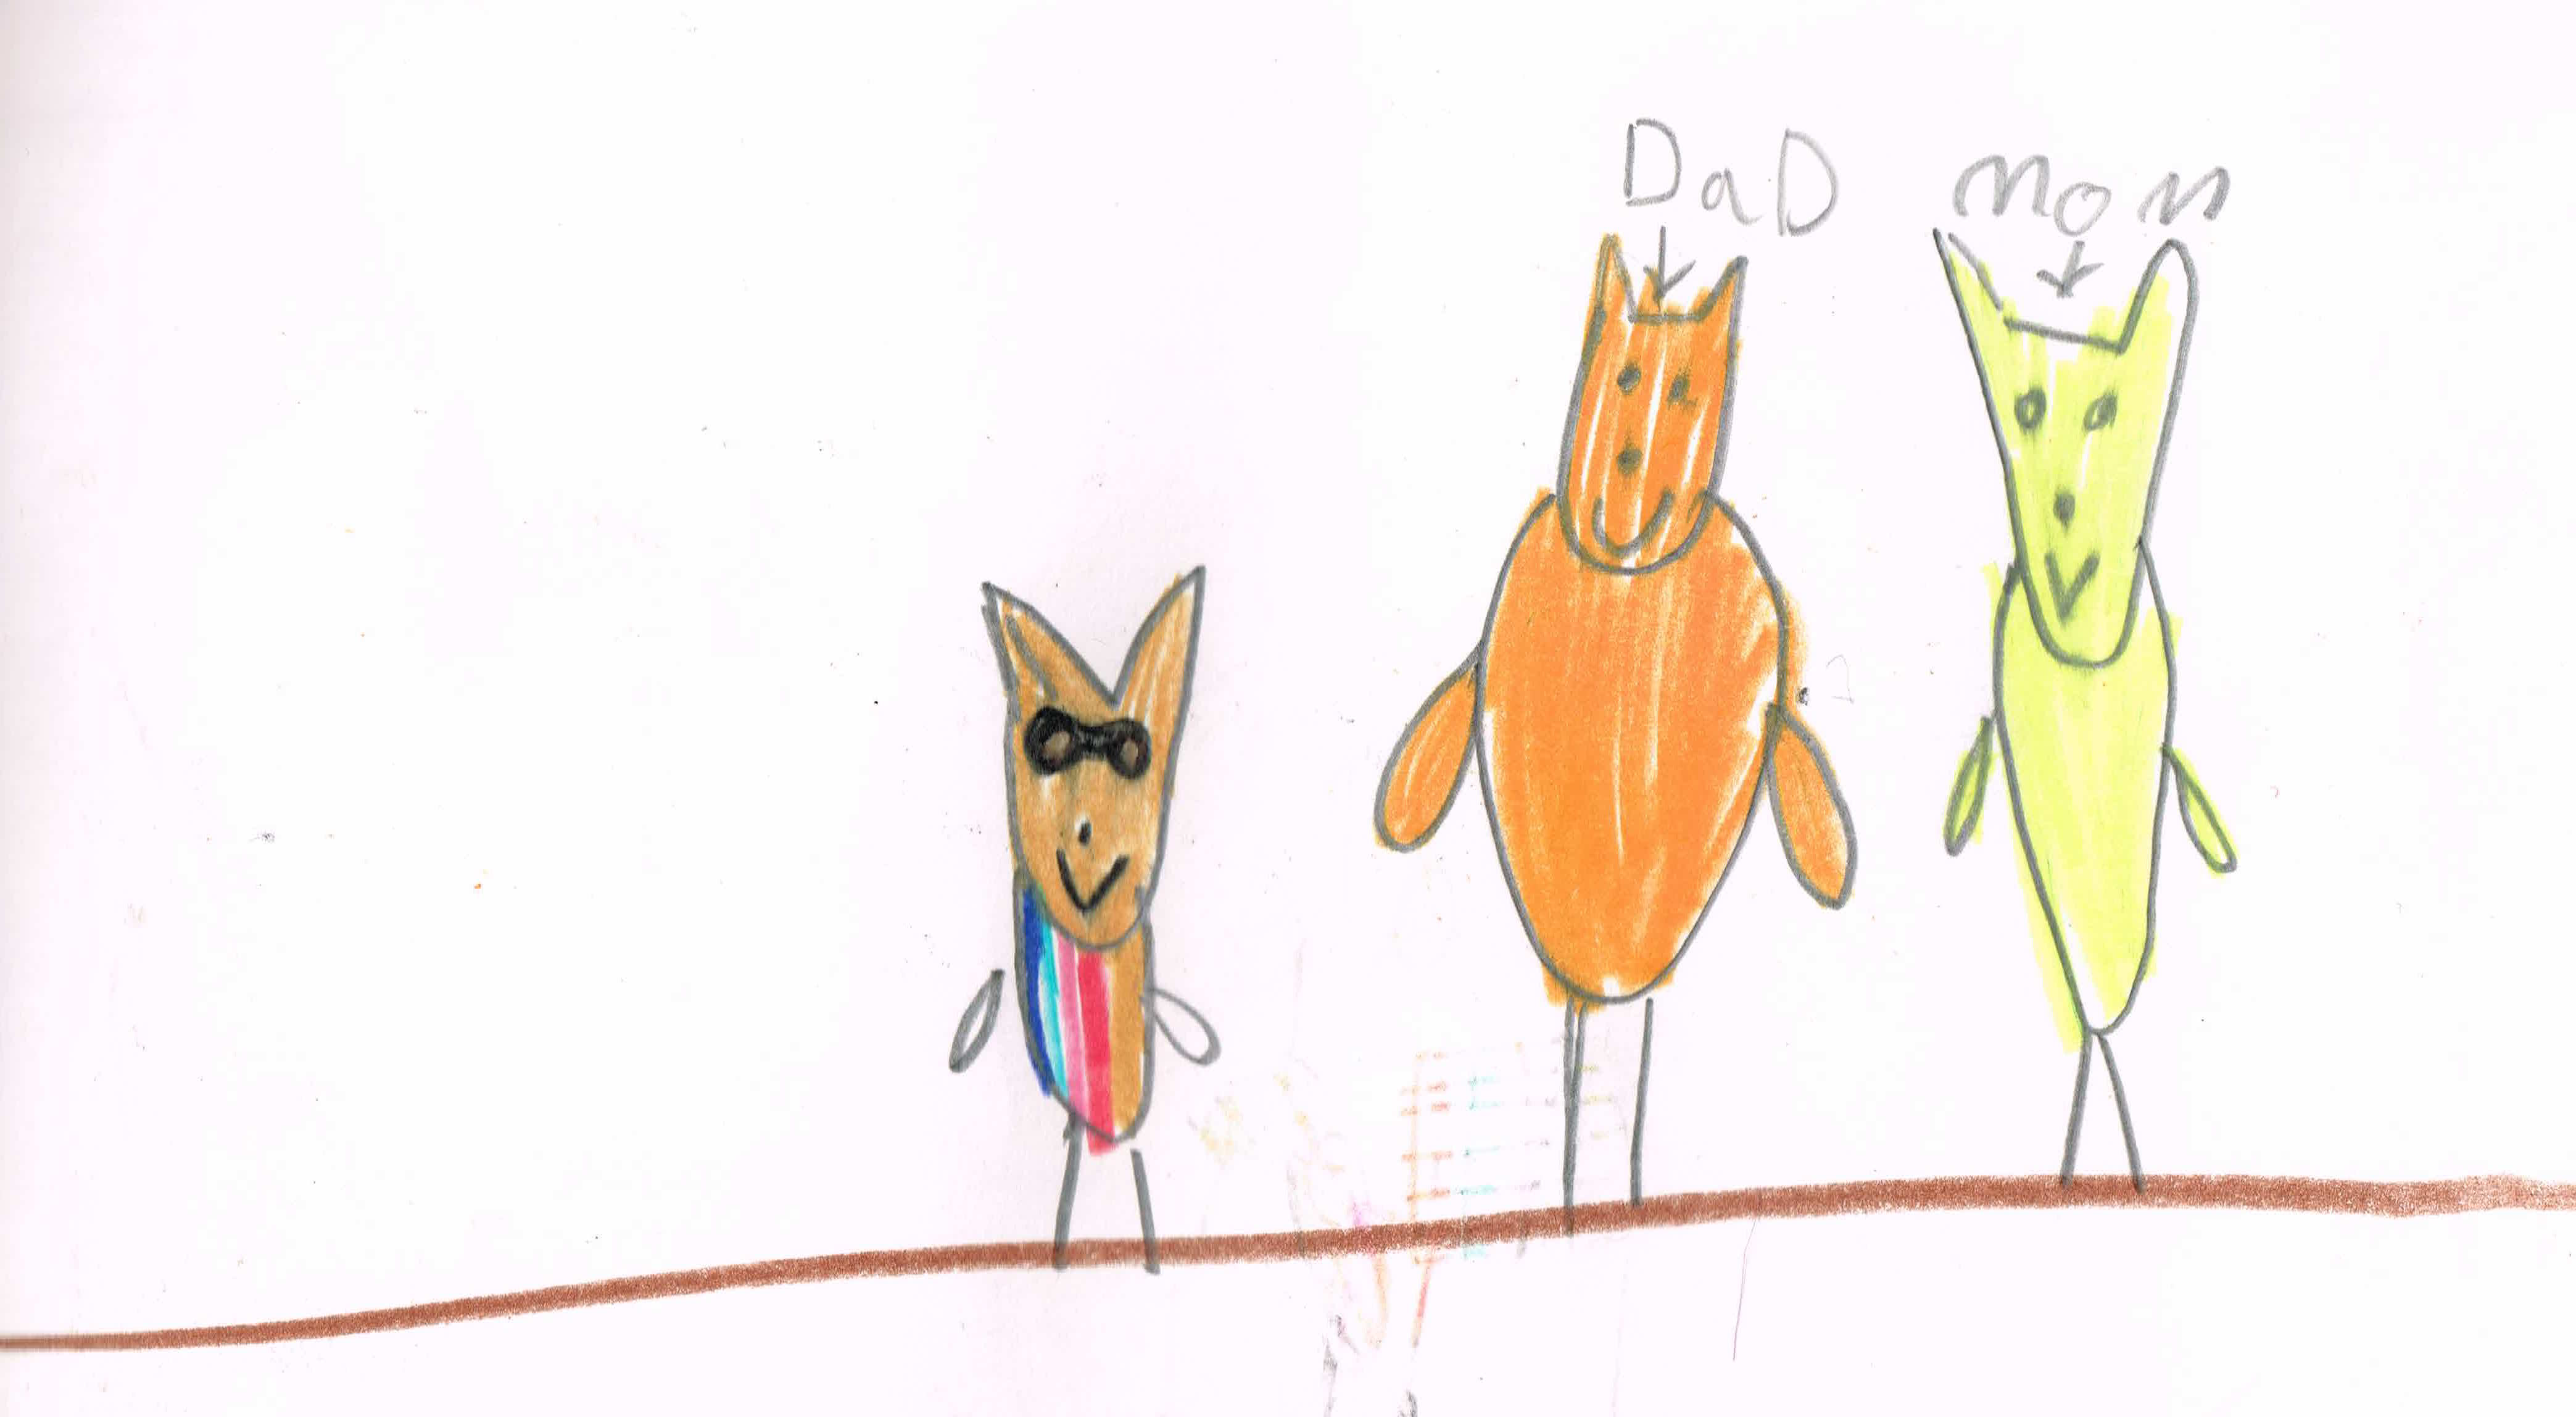
\includegraphics[width=\textwidth]{img/cm-pic02.png}
\end{center}
  
  Her parents kept reassuring her that she would make a friend some night.
  But Cora was sure that they were just saying that to make her feel good.

\pagebreak  

  Then one night, she was playing a lonely game of checkers all by
  herself. Then there was a dreadful crashing sound. The crash was coming
  from her favorite blue house in the town.
  
\begin{center}
  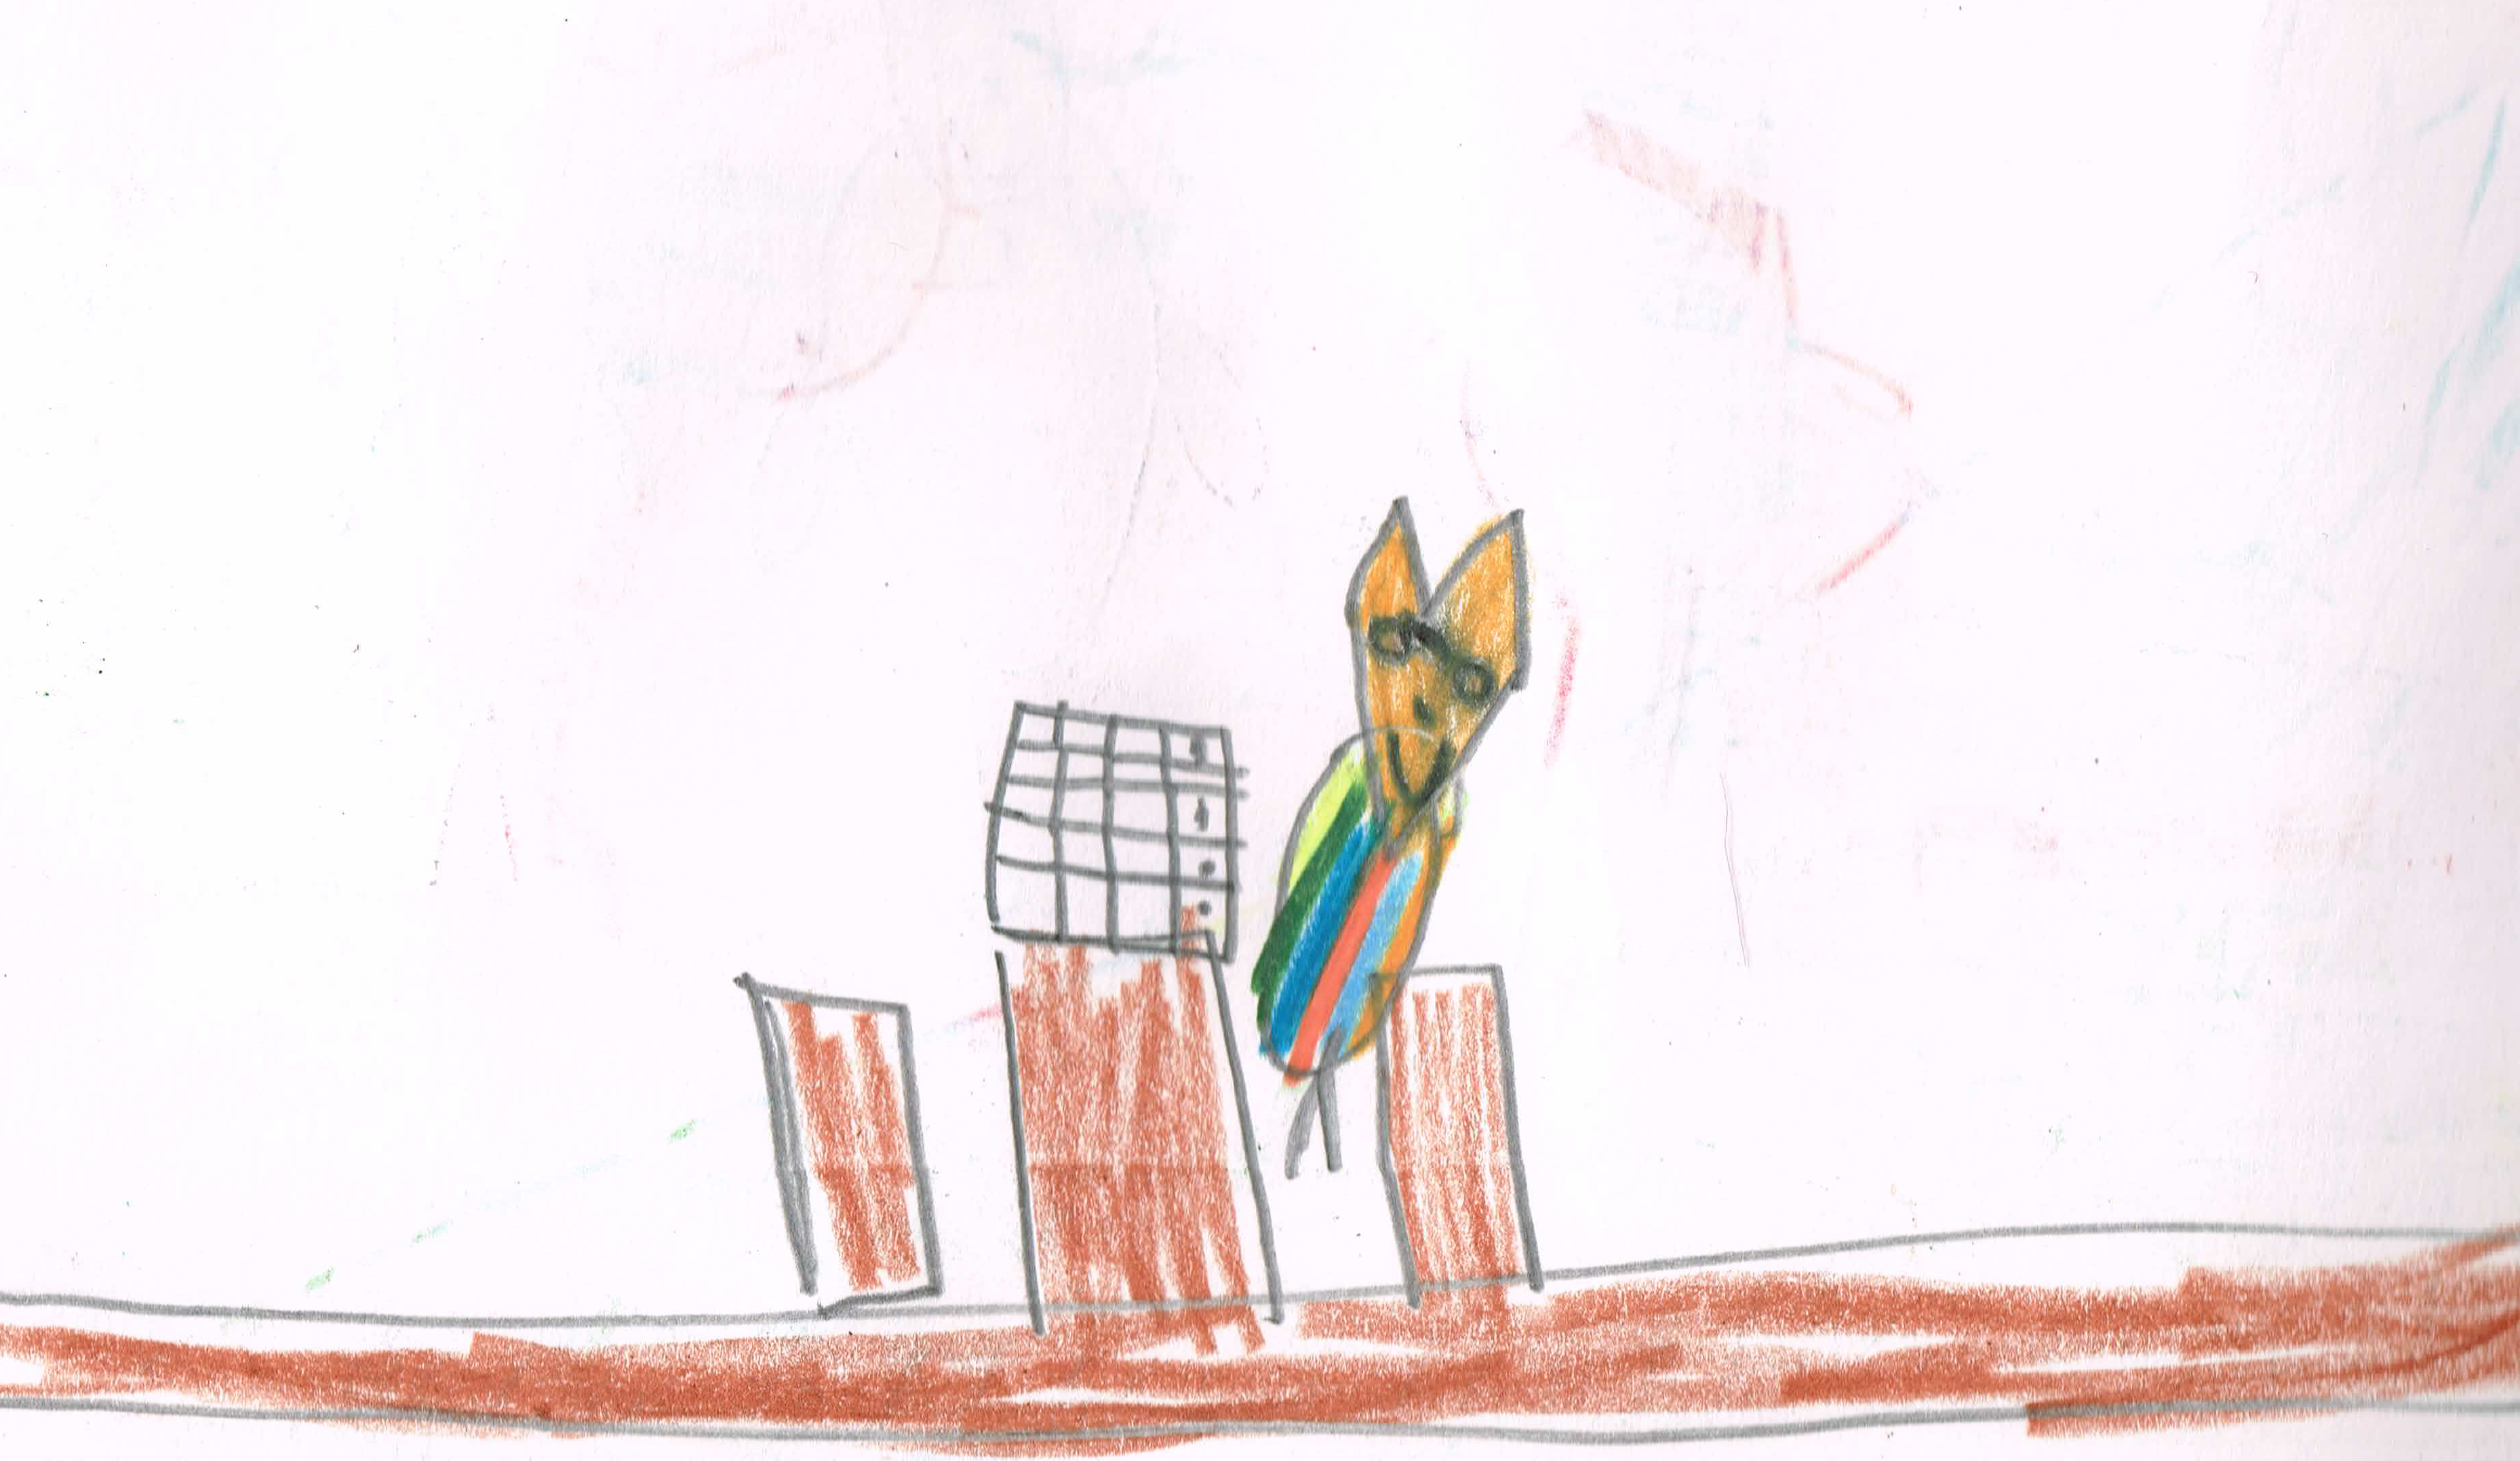
\includegraphics[width=\textwidth]{img/cm-pic03.png}
\end{center}
  
\pagebreak

  $\ $\vfill  
  \includegraphics[width=\textwidth]{img/cm-pic04.png}
  \vfill

\pagebreak

$\ $\vspace{1cm}

  She flew over to the house and landed on the roof. The roof wasn't the
  most comfortable place in the world, but it would do for now. She peered
  down and saw that the trash cans were knocked over. So she just walked
  away slowly. But WAIT! She turned around as fast as lightning because
  she just saw a flashback of right before she started the game of
  checkers (which was about 20 minutes ago). In her flashback, she saw
  that the trash cans weren't knocked over. So she said to herself,
  \enquote{I shall just take a tiny peek.}
  \vfill

\pagebreak

\begin{center}
  $\ $\vfill
  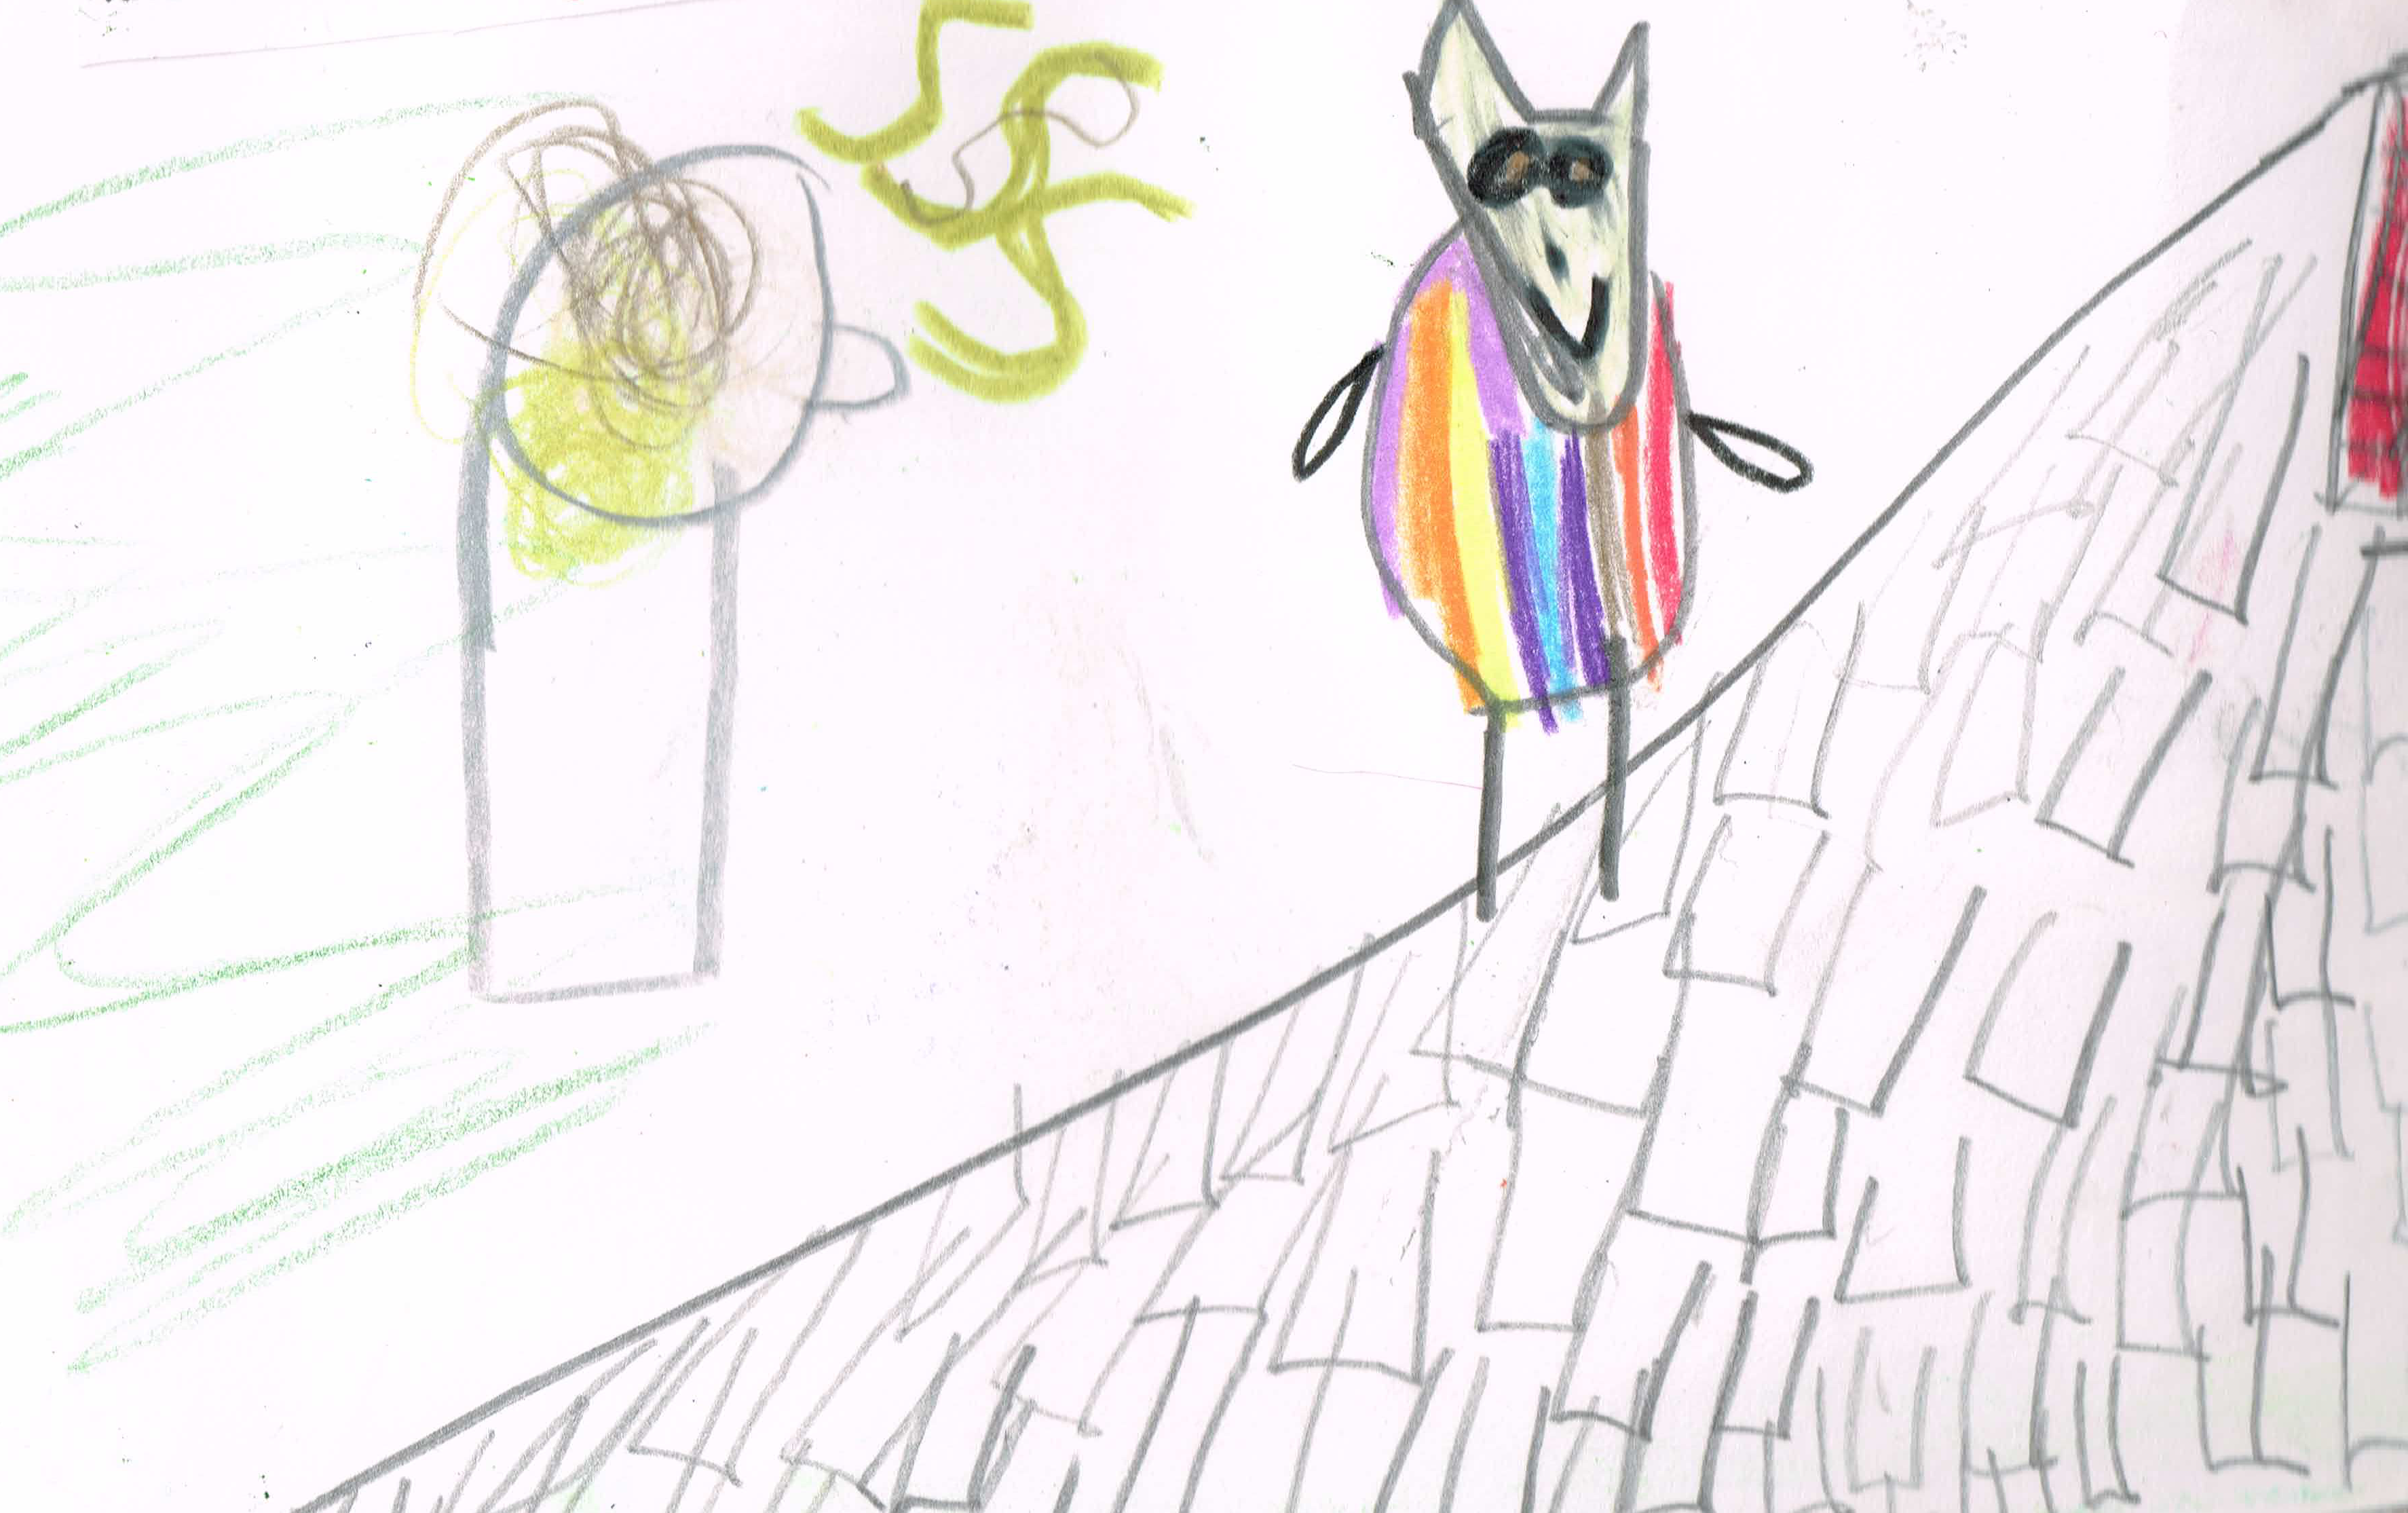
\includegraphics[width=\textwidth]{img/cm-pic05.png}
  \vfill
\end{center}

\pagebreak
  
  So she peered again over the edge and then she saw, out of the bushes, a
  tiny black nose as small as a button. And then a bigger head! And on
  that head, there was gray fur. Around the eyes there was dark black fur
  in the shape of a mask! Just like hers!
  
\begin{center}
  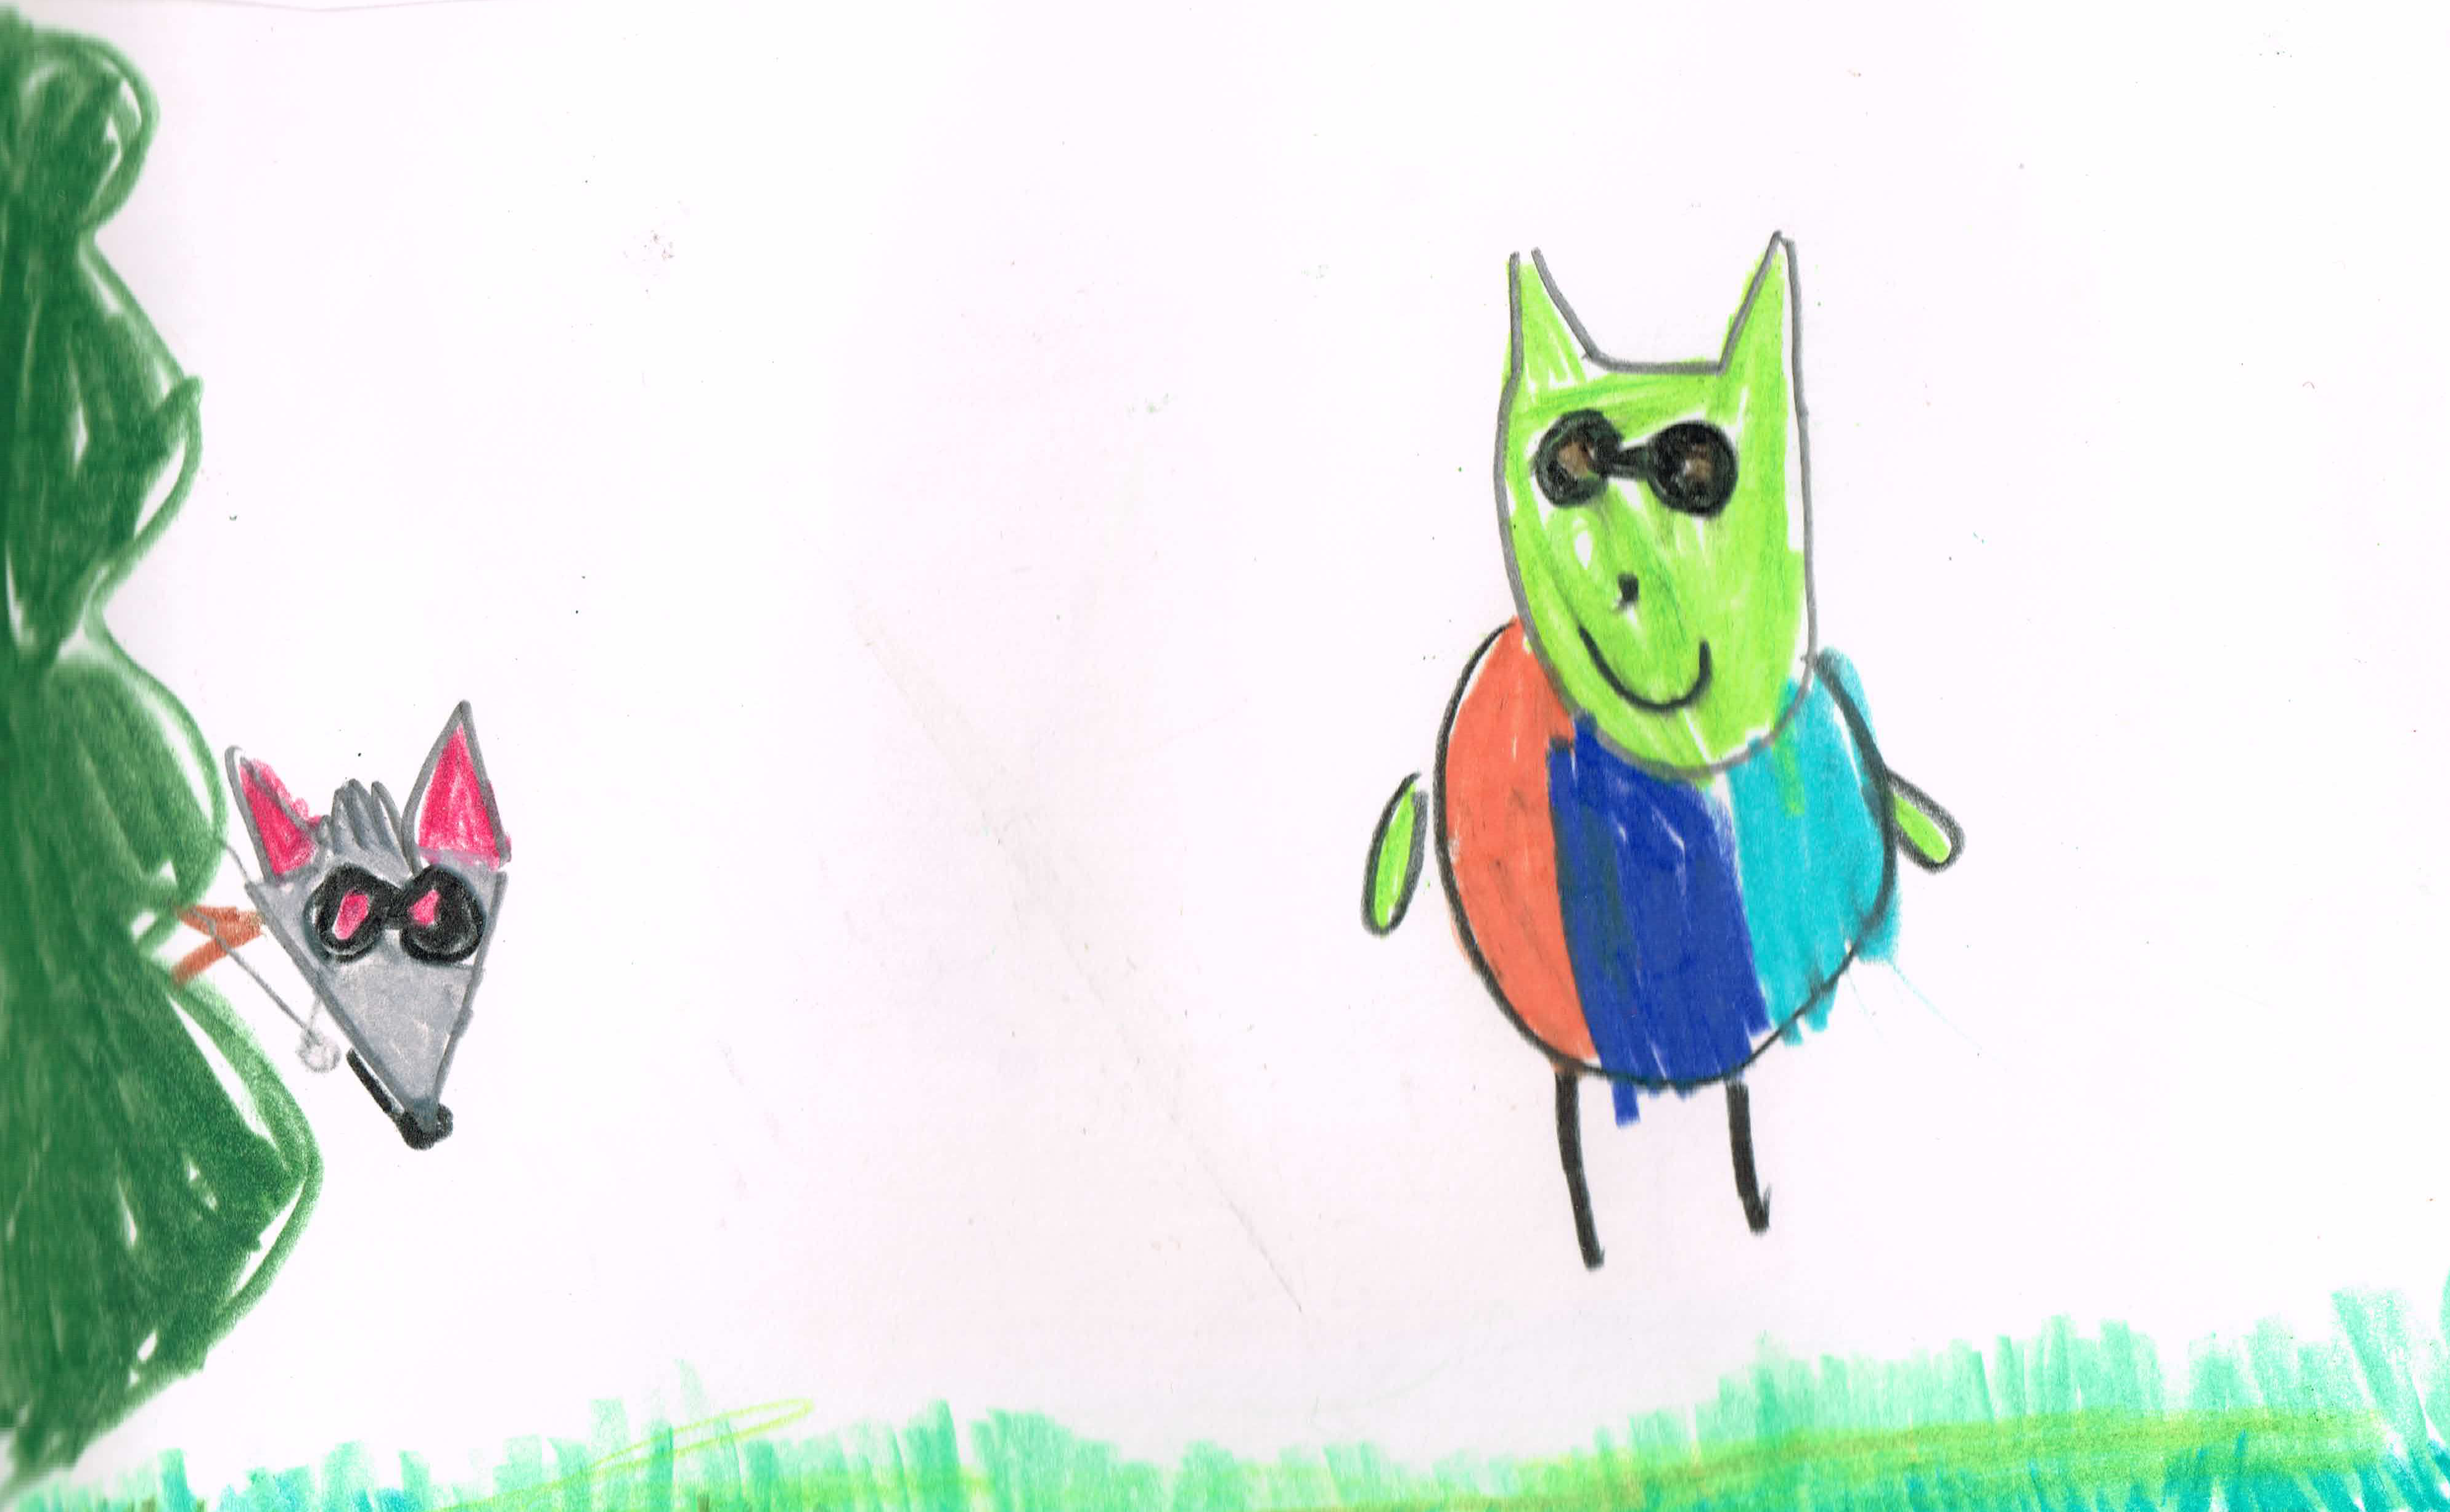
\includegraphics[width=\textwidth]{img/cm-pic06.png}
\end{center}

\pagebreak  
  
  Cora had never been so excited in her life! She flew down and landed on
  the ground and then walked quietly to the peculiar creature. Not wanting
  to frighten it, she said in her quietest voice - but not too quiet -
  \enquote{my name is Cora. What is yours?} The peculiar creature looked
  up and said, \enquote{You're an owl, aren't you?} \enquote{Yes, I'm an
  owl,} replied Cora. \enquote{And a very pretty owl!} replied the
  peculiar creature. \enquote{I guess you should know what I am if we are
  going to be friends.} Cora the owl said, \enquote{We're going to be
  friends?} Her eyes filled with tears from excitement. Then Cora asked,
  \enquote{will you please tell me what you are?} The creature replied,
  \enquote{of course, I will. I am a raccoon. And my name is Mary. And I
  have a very unique birthmark too.} Mary came all the way out of the
  bushes, slowly, careful not to wake the human beings. Cora was amazed at
  what she saw on the raccoon. Mary was colorful, bright and beautiful with
  what looked like feathers but was fur.

\pagebreak
  
  $\ $\vfill  
  \includegraphics[width=\textwidth]{img/cm-pic07.png}
  \vfill

\pagebreak

  \enquote{Tonight, do you want to have a slumber party and stay up late
  and watch what humans call the sunrise?} asked Cora. Mary replied,
  \enquote{I would LOVE to! I've never been invited to a slumber party!}
  
\begin{center}
  \includegraphics[width=\textwidth]{img/cm-pic08.png}
\end{center}
  

\pagebreak
  
\begin{center}
  \includegraphics[width=\textwidth]{img/cm-pic09.png}
\end{center}
\vfill  
  That is how Cora and Mary became friends.
\vfill

\pagebreak
  
  $\ $\vfill  
  \includegraphics[width=\textwidth]{img/cm-pic10.png}
  \vfill  

\pagebreak
  
  $\ $\vfill  
  \includegraphics[width=\textwidth]{img/cm-pic11.png}
  \vfill  

\pagebreak

  The company publishing this book wanted more pages. So, we added a portion for you to write the next chapter in the friendship of Cora and Mary. Write your own story about the next day or even the next adventure. Enjoy!

  \gl 5 4

\pagebreak

  \gl 7 6

\pagebreak

  \gl 7 6

\pagebreak

  \gl 7 6

\pagebreak

  \gl 7 6

\pagebreak

  \gl 7 6

\pagebreak

  \gl 7 6

\pagebreak

  \gl 7 6

\pagebreak

  \gl 7 6

\pagebreak

  \gl 7 6




\end{document}

